\documentclass[aspectratio=169]{beamer}
\usepackage[utf8]{inputenc}
\usepackage[T1]{fontenc}
\usepackage[brazil]{babel}
\usepackage{ragged2e}
\usepackage{booktabs}
\usepackage{verbatim}
\usetheme{AnnArbor}
\usecolortheme{orchid}
\usefonttheme[onlymath]{serif}
\usepackage{listings}

\lstset{language=C,
	backgroundcolor=\color{green!10},
	basicstyle=\ttfamily,
	keywordstyle=\color{blue}\ttfamily,
	stringstyle=\color{red}\ttfamily,
	commentstyle=\color{green}\ttfamily,
	morecomment=[l][\color{magenta}]{\#}
}

\AtBeginSection[]{
  \begin{frame}
  \vfill
  \centering
  \begin{beamercolorbox}[sep=8pt,center,shadow=true,rounded=true]{title}
    \usebeamerfont{title}\insertsectionhead\par%
  \end{beamercolorbox}
  \vfill
  \end{frame}
}

\title[\sc{ALEST I - Apresentação da Disciplina e Revisão}]{Algoritmos e Estruturas de Dados I - Apresentação da Disciplina e Revisão}
\author[Roland Teodorowitsch]{Roland Teodorowitsch}
\institute[ALEST I - EP - PUCRS]{Algoritmos e Estruturas de Dados I - Escola Politécnica - PUCRS}
\date{31 de julho de 2023}

\begin{document}
\justifying

%-------------------------------------------------------
\begin{frame}
	\titlepage
\end{frame}

%=======================================================
\section{Apresenta\c{c}\~ao da Disciplina}

%-------------------------------------------------------
\begin{frame}\frametitle{Sobre o professor}
\begin{itemize}
	\item Nome:
		\begin{itemize}
			\item Roland Teodorowitsch
		\end{itemize}
	\item Forma\c{c}\~ao:
		\begin{itemize}
			\item Bel. em Inform\'atica (PUCRS, 1990)
			\item Msc. em Ci\^encia da Computa\c{c}\~ao (UFRGS, 1994)
		\end{itemize}
	\item \'Areas de Interesse:
		\begin{itemize}
			\item SD, SO, STR, PP, Sist. Embarc., Arq. de Comp.
		\end{itemize}
	\item E-mail:
		\begin{itemize}
			\item roland.teodorowitsch@pucrs.br
		\end{itemize}
\end{itemize}
\end{frame}

%-------------------------------------------------------
\begin{frame}\frametitle{Sobre a disciplina}
\begin{itemize}
	\item Nome: Algoritmos e Estruturas de Dados I
	\item Código: 4645G-04
	\item Turma: 14
	\item Cr\'editos: 4
	\item Carga-horária: 60 horas-aula
	\item Hor\'ario: 3CD 5CD (CD=9h45min-11h15min)
	\item Modalidade: presencial
\end{itemize}
\end{frame}

%-------------------------------------------------------
\begin{frame}\frametitle{Sobre a disciplina}
\begin{itemize}
	\item Semestre: 2
	\item Pré-requisito:
		\begin{itemize}
			\item Introdução à Programação - ECo ou Fundamentos de Programação
		\end{itemize}
	\item Co-requisito:
		\begin{itemize}
			\item Programação Orientada a Objetos - ECo ou Programação Orientada a Objetos
		\end{itemize}
	\item É pré-requisito para:
		\begin{itemize}
			\item Algoritmos e Estruturas de Dados II
		\end{itemize}
\end{itemize}
\end{frame}

%-------------------------------------------------------
\begin{frame}\frametitle{Objetivos}
O aluno ao término da disciplina deverá ser capaz de:
\begin{enumerate}
	\item Conhecer e utilizar as técnicas fundamentais para avaliar a complexidade de algoritmos.
	\item Conhecer e diferenciar as estruturas de dados: listas, filas, pilhas e árvores.
	\item Manipular estas estruturas de dados por meio de algoritmos.
	\item Selecionar e construir estruturas de dados adequadas para aplicações específicas, bem como modelar estas aplicações.
	\item Aplicar algoritmos de ordenação e de pesquisa na solução de problemas.
\end{enumerate}
\end{frame}

%=======================================================
\section{Conte\'udo}
	
%-------------------------------------------------------
\begin{frame}\frametitle{Ementa}
Construção e raciocínio sobre diferentes algoritmos e implementações para estruturas de dados lineares e hierárquicas: listas, filas, pilhas e árvores. Exame da adequação destes algoritmos na solução de diversas classes de problemas. Construção de algoritmos e implementações para problemas de ordenação e pesquisa. Discussão, análise e raciocínio sobre a complexidade de algoritmos e implementações correspondentes.
\end{frame}

%-------------------------------------------------------
\begin{frame}\frametitle{Conte\'udo (1/4)}
4 grandes unidades
\begin{itemize}
	\item Complexidade de algoritmos
	\item Estruturas lineares
	\item Classificação e pesquisa
	\item Árvores
\end{itemize}
\end{frame}

%-------------------------------------------------------
\begin{frame}\frametitle{Conte\'udo (2/4)}
\small{1. Complexidade de algoritmos\\
~ 1.1. Contagem de operações\\
~ 1.2. Notação O\\
~\\
2. Estruturas lineares\\
~ 2.1. Estruturas contíguas X Estruturas encadeadas\\
~ 2.2. Coleções e suas operações de acesso\\
~ ~ 2.2.1. Listas\\
~ ~ 2.2.2. Pilhas\\
~ ~ 2.2.3. Fila}
\end{frame}

%-------------------------------------------------------
\begin{frame}\frametitle{Conte\'udo (2/4)}
\small{3. Classificação e pesquisa\\
~ 3.1. Pesquisa sequencial X pesquisa binária\\
~ 3.2. Classificação de dados\\
~ ~ 3.2.1. Bubble Sort\\
~ ~ 3.2.2. Insertion Sort\\
~ ~ 3.2.3. Mergesort\\
~ ~ 3.2.4. Quicksort\\
~\\
4. Árvores\\
~ 4.1. Definições e representação\\
~ 4.2. Árvores genéricas\\
~ 4.3. Árvores binárias de pesquisa\\
~ 4.4. Operações: caminhamento, pesquisa, inserção, remoção\\
~ 4.5. Árvores balanceadas e sua eficiência}
\end{frame}

%-------------------------------------------------------
\begin{frame}\frametitle{Bibliografia Básica}
CORMEN, T. H. \textbf{Algoritmos - teoria e prática}. 3 ed., Rio de Janeiro: Elsevier-Campus, 2012.\\
~\\
ELLIS, H.; SAHNI, S.; RAJASEKARAN, S. \textbf{Computer algorithms}. Silicon Press, 2007.\\
~\\
GOODRICH, M. T.; TAMASSIA, R. \textbf{Estruturas de dados e algoritmos em Java}. 5 ed., Porto Alegre: Bookman, 2013.
\end{frame}

%-------------------------------------------------------
\begin{frame}\frametitle{Bibliografia Complementar}
SEDGEWICK, Robert. \textbf{Algorithms in C++}. 3rd ed., Boston: Addison-Wesley, 1998. ISBN: 0201350882.\\
~\\
MCALLISTER, W. \textbf{Data structures and algorithms using Java}. Boston: Jones and Bartlett, 2009.\\
~\\
SEDGEWICK, Robert; WAYNE, Kevin. \textbf{Algorithms, Fourth Edition}. Addison-Wesley Professional, 4th ed., 2011. ISBN-10: 032157351X.\\
~\\
SZWARCFITER, Jayme L.; MARKENZON, Lilian.
\textbf{Estruturas de Dados e Seus Algoritmos}.
LTC, 3rd edição, Grupo GEN, 2010.
ISBN: 978-85-216-2994-8.\\
~\\
AHO, A. V. \textbf{Foundations of computer science}. New York: Computer Science Press, 1998.
\end{frame}

%=======================================================
\section{Avalia\c{c}\~ao}

%-------------------------------------------------------
\begin{frame}\frametitle{Avalia\c{c}\~ao}
\[
G1 = \frac{MT  + P_1 + P_2}{3}
\]
\begin{itemize}
	\item $MT$ = média dos trabalhos do semestre, podendo permitir pesos diferentes entre os trabalhos
	\item $P_1$ = prova sobre os conteúdos das unidades 1, 2 e 3
	\item $P_2$ = prova sobre todo o conteúdo da disciplina
\end{itemize}
\end{frame}
	
%-------------------------------------------------------
\begin{comment}
\begin{frame}\frametitle{Trabalhos}
	\begin{itemize}
		\item $T_1$ = Trabalho de ...
		\begin{itemize}
			\item 2023/2: ...
		\end{itemize}
		\item $T_2$ = Trabalho de ...
		\begin{itemize}
			\item 2023/2: ...
		\end{itemize}
\end{frame}
\end{comment}

%-------------------------------------------------------
\begin{comment}
\begin{frame}\frametitle{\'Indices de Aprova\c{c}\~ao}
	\begin{table}
		\centering
		\begin{tabular}{cccccccc}
			\toprule
			SEM. & N\'UM. AL. & APROV. & REP. & REP. FALTAS & CANC. & CANC. NC\\
			\midrule
			2023/2 & 0 & 0 (0,0\%) & 0 (0,0\%) & 0 (0,0\%) & 0 (0,0\%)& 0 (0,0\%)\\
			\bottomrule
		\end{tabular}
		\caption{\'Indices de Aprova\c{c}\~ao}
	\end{table}
\end{frame}
\end{comment}

%=======================================================
\section{Informa\c{c}\~oes Gerais}

%-------------------------------------------------------
\begin{frame}\frametitle{Avisos: Presenças e Faltas}
\begin{itemize}
	\item 1 encontro = 2 presen\c{c}as ou faltas
	\item em 2023-2: 34 encontros (68 horas/aula) com presença contabilizada
	\item na semana de G2, a presença NÃO é contabilizada
	\item frequ\^encia m\'inima para aprova\c{c}\~ao: 75\%
	\item limite de faltas = 25\% de 68 = 17
	\item portanto, com 18 faltas (9 encontros) o aluno está REPROVADO POR FALTAS
\end{itemize}
\end{frame}

%-------------------------------------------------------
\begin{frame}\frametitle{Avisos: Moodle}
\begin{itemize}	
	\item Avisos pelo Mural
	\item D\'uvidas pelo f\'orum
	\item Material de apoio
	\item Entrega de trabalhos e exerc\'icios
\end{itemize}
\end{frame}

%-------------------------------------------------------
\begin{frame}\frametitle{Avisos: Diversos}
\begin{itemize}
	\item Listas de exercícios com múltiplas entregas
%	\item Avaliação personalizada
\end{itemize}
\end{frame}

%-------------------------------------------------------
\begin{frame}\frametitle{Avisos: Mapas Mentais}
\begin{itemize}
	\item São uma forma de representar conhecimento sobre determinado assunto
	\item Recomenda-se fortemente que o aluno construa Mapas Mentais dos conteúdos da disciplina
	\item Os Mapas Mentais poderão ser usados nas avaliações da disciplina (com exceção das provas PS e G2)
	\item Regras:
	\begin{itemize}
		\item Um Mapa Mental por unidade do conteúdo programático
		\item NÃO incluir textos grandes e/ou copiados e colados nos nodos do mapa
		\item Cada Mapa Mental em uma folha A4 impressa
		\item Todos os Mapas Mentais devem ser entregues uma semana antes da avaliação em que serão utilizados
	\end{itemize}
	\item Mapas Conceituais também são uma alternativa interessante
\end{itemize}
\end{frame}

%-------------------------------------------------------
\begin{frame}\frametitle{Avisos: Recomendações}
\begin{itemize}
	%\item Realizar as leituras indicadas antes da aula
	\item Dificuldades não esclarecidas em disciplinas anteriores NÃO serão resolvidas sem esforço adicional
	\item Consultem as obras disponíveis na biblioteca (livros físicos e on-line)
	\item Aproveitar a aula para realizar os exercícios
	\item Não deixe acumular trabalhos
	\item Não se aprende a programar estudando na véspera da prova...
	\item Reserve um horário de estudo na semana para cada uma das disciplinas
	\item "Disciplina é liberdade..." (letra da música Há Tempos, da banda Legião Urbana)
	\item Existe uma monitoria que presta apoio aos alunos com dúvidas (verifique horários na página de monitoria)
\end{itemize}
\end{frame}

\begin{comment}
%-------------------------------------------------------
\begin{frame}\frametitle{Avisos: Diversos}
\begin{itemize}
    \item Em todos os horários da disciplina, o professor estará \emph{on-line} no Zoom
    \item Na maioria dos tópicos, haverá uma aula expositiva (via Zoom ou via vídeo disponibilizado no YouTube) seguida de uma aula de exercícios para entrega
    \item No moodle, há um \emph{link} com convite para o grupo de Whatsapp
%	\item Método 300
%	\item Presenças e faltas devem ser acompanhadas pelo aplicativo
%	\item Avaliação personalizada
\end{itemize}
\end{frame}
\end{comment}

%=======================================================
\section{Dúvidas?}

%-------------------------------------------------------
\begin{frame}\frametitle{Dúvidas?}
	\begin{figure}[h]
		\centering
		
\includegraphics[height=0.6\paperheight]{pucrs-ec-poo-unidade_00-apresentacao_da_disciplina_e_revisao-laminas-duvidas.png}
	\end{figure}
\end{frame}

%=======================================================
\section{Mensagens Finais}

\begin{comment}
%-------------------------------------------------------
\begin{frame}\frametitle{Mensagens Finais}
	\begin{figure}[h]
		\centering
		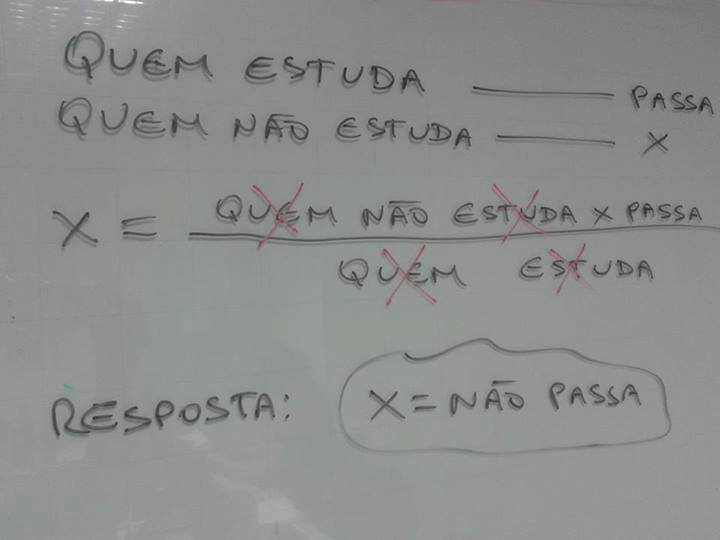
\includegraphics[height=0.6\paperheight]{pucrs-ec-poo-unidade_00-apresentacao_da_disciplina_e_revisao-laminas-quem_estuda.jpg}
		\caption{https://www.facebook.com/acreditesouengenheiro}\label{quemEstuda}
	\end{figure}
\end{frame}
\end{comment}

%-------------------------------------------------------
\begin{frame}\frametitle{Mensagens Finais}
	\begin{block}{Plat\~ao}
		O objetivo da educação é o de nos ensinar a amar a beleza.
	\end{block}
	\begin{block}{Aristóteles}
		A educação tem raízes amargas, mas os seus frutos são doces.\\
		~\\
		É fazendo que se aprende a fazer aquilo que se deve aprender a fazer.\\
		~\\
		A alegria que se tem em pensar e aprender faz-nos pensar e aprender ainda mais.\\
		~\\
		A primeira qualidade do estilo é a clareza.
	\end{block}
\end{frame}

%-------------------------------------------------------
\begin{frame}\frametitle{Mensagens Finais}
	\begin{block}{Albert Einstein}
		A única coisa que interfere com meu aprendizado é a minha educação.
	\end{block}
	\begin{block}{Ralph Waldo Emerson}
		O que é ensinado em escolas e universidades não representa educação, mas são meios para obtê-la.
	\end{block}
	\begin{block}{Derek Bok}
		Se você acha que educação é cara, experimente a ignorância.
	\end{block}
\end{frame}

%-------------------------------------------------------
\begin{frame}\frametitle{Mensagens Finais}
	\begin{block}{Cora Coralina}
		Feliz aquele que transfere o que sabe e aprende o que ensina.
	\end{block}
	\begin{block}{Guimarães Rosa}
		Mestre não é quem sempre ensina, mas quem de repente aprende.
	\end{block}
\end{frame}

%-------------------------------------------------------
\begin{frame}\frametitle{Bem-vindos}
	\begin{figure}[h]
		\centering
		
\includegraphics[height=0.7\paperheight]{pucrs-ec-poo-unidade_00-apresentacao_da_disciplina_e_revisao-laminas-welcome.jpg}
	\end{figure}
\end{frame}

%=======================================================
\section{Revisão}

%-------------------------------------------------------
\begin{frame}[fragile]\frametitle{Introdução à Prog. (EC) - Prova P3 - 2022/1 - Prof. João B. Oliveira}

\begin{enumerate}
	\item Escreva uma função que recebe um vetor de inteiros, seu tamanho, um valor {\tt val} e troca todas as ocorrências de {\tt val} no vetor por {\tt val+1}, exceto a última ocorrência.
	\item Escreva uma função que recebe o nome de um arquivo que contém inteiros e examina o arquivo, imprimindo o maior inteiro que estiver nele. Você não sabe quantos inteiros estão no arquivo.
	\item Para esta questão, suponha que você tem a struct
{\scriptsize
\begin{lstlisting}
struct data {
  int dia, mes, ano;
};
\end{lstlisting}}
Escreva uma função que recebe duas datas {\tt d1} e {\tt d2} e imprime a mais antiga delas. Suponha que já existe uma função {\tt printdata()} que pode ser usada.
\end{enumerate}
\end{frame}

%-------------------------------------------------------
\begin{frame}[fragile]\frametitle{Introdução à Prog. (EC) - Prova P3 - 2022/1 - Prof. João B. Oliveira}
\begin{enumerate}
\setcounter{enumi}{3}
\item Escreva uma função que recebe um vetor de números inteiros e o seu tamanho e verifica se algum número que está no vetor é a soma de outros dois números do vetor. 
 \item Para as questões abaixo, suponha que você já tem a struct a seguir:
{\tiny
\begin{lstlisting}
  struct data {
    int dia, mes, ano;
  };

  struct pessoa {
    char nome[40];
    struct data nasc, admissao, saida;
    int identidade, cpf;
  };
\end{lstlisting}}
e também um vetor de funcionários
{\tiny
\begin{lstlisting}
struct pessoa funcs[50];
\end{lstlisting}}
Escreva um algoritmo que imprime uma lista de todas as pessoas que nasceram em maio. E também um algoritmo que recebe o cpf de uma pessoa e imprime seu nome se ele é funcionário da empresa.
\end{enumerate}
\end{frame}

%-------------------------------------------------------
\end{document}

